\section{Introduction}

Model-based metrics for evaluating machine translation such as BLEURT \cite{sellam-etal-2020-bleurt}, ESIM \cite{mathur-etal-2019-ESIM}, and YiSi \cite{lo-2019-yisi} have recently attracted attention due to their superior correlation with human judgments \cite{WMT19-metrics-proceedings}. However, \bleu~\cite{papineni-etal-2002-bleu} remains  the most widely used corpus-level MT metric. It correlates reasonably well with human judgments, and moreover is easy to understand and cheap to calculate, requiring only reference translations in the target language. By contrast, model-based metrics require tuning on thousands of examples of human evaluation for every new target language or domain \cite{sellam-etal-2020-bleurt}. Model-based metric scores are also opaque and can hide undesirable biases, as can be seen in Table~\ref{tab:bleurt-bias}.


\begin{table}[ht]
    \centering
    \footnotesize
    \begin{tabular}{l l l }
Reference:& \multicolumn{2}{l}{You must be a doctor.} \\
Hypothesis: & \multicolumn{2}{l}{$\rule{1cm}{0.15mm}$ must be a doctor.} \\
    % & You &	~0.990 \\
    & He	&-0.735 \\
    %& Alexandra & -0.888 \\
    %& Alexander & -0.975 \\
    & Joe & -0.975 \\
    & Sue & -1.043 \\
    & She	 &-1.100 \\\hline
Reference:& \multicolumn{2}{l}{It is the greatest country in the world.} \\
Hypothesis:& \multicolumn{2}{l}{$\rule{1cm}{0.15mm}$ is the greatest country in the world.} \\
    % & It	& ~0.957 \\
    & France &	-0.022 \\
    & America	& -0.060 \\
    & Russia &	-0.161 \\
    %& China  & -0.166 \\
    %& USA    & -0.168 \\
    %& India   &	-0.211 \\
    & Canada  & -0.309 
    \end{tabular}
    \caption{A demonstration of BLEURT's internal biases; model-free metrics like BLEU would consider each of the errors above to be equally wrong.}
    \label{tab:bleurt-bias}
\end{table}

The source of model-based metrics' (e.g. BLEURT) correlative superiority over model-free metrics (e.g. BLEU) appears to be the former's ability to focus evaluation on \textit{adequacy}, while the latter are overly focused on \textit{fluency}. BLEU and most other generation metrics consider each output \textit{token} equally. Since natural language is dominated by a few high-count types, an MT model that concentrates on getting its \textit{if}s, \textit{and}s and \textit{but}s right will benefit from BLEU in the long run more than one that gets its \textit{xylophone}s, \textit{peripatetic}s, and \textit{defenestrate}s right. Can we derive a metric with the discriminating power of BLEURT that does not share its bias or expense and is as interpretable as BLEU? 

As it turns out, the metric may already exist and be in common use. Information extraction and other areas concerned with classification have long used both \textit{micro averaging}, which treats each token equally, and \textit{macro averaging}, which instead treats each \textit{type} equally, when evaluating. The latter in particular is useful when seeking to avoid results dominated by overly frequent types.  In this work we take a classification-based approach to evaluating machine translation in order to obtain an easy-to-calculate metric that focuses on adequacy as much as BLEURT but does not have the expensive overhead, opacity, or bias of model-based methods. 


% \begin{figure}[ht!]
%     \centering
%     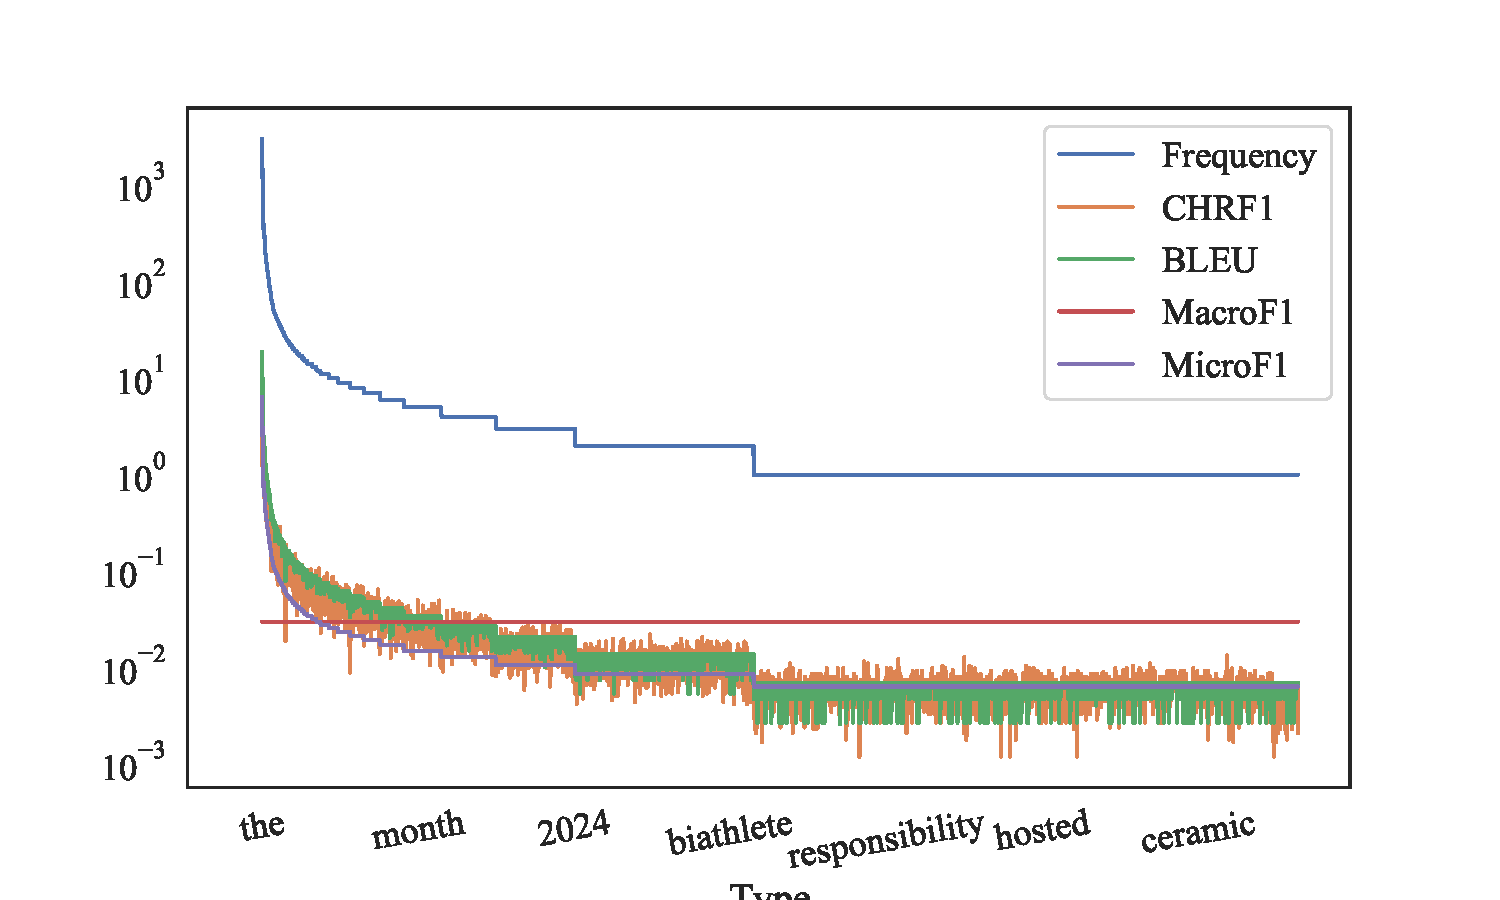
\includegraphics[width=\linewidth,trim={15mm 5mm 25mm 15mm},clip]{img/bleu-chrf-macro-micro-swapin-lenmatch.pdf}
%     %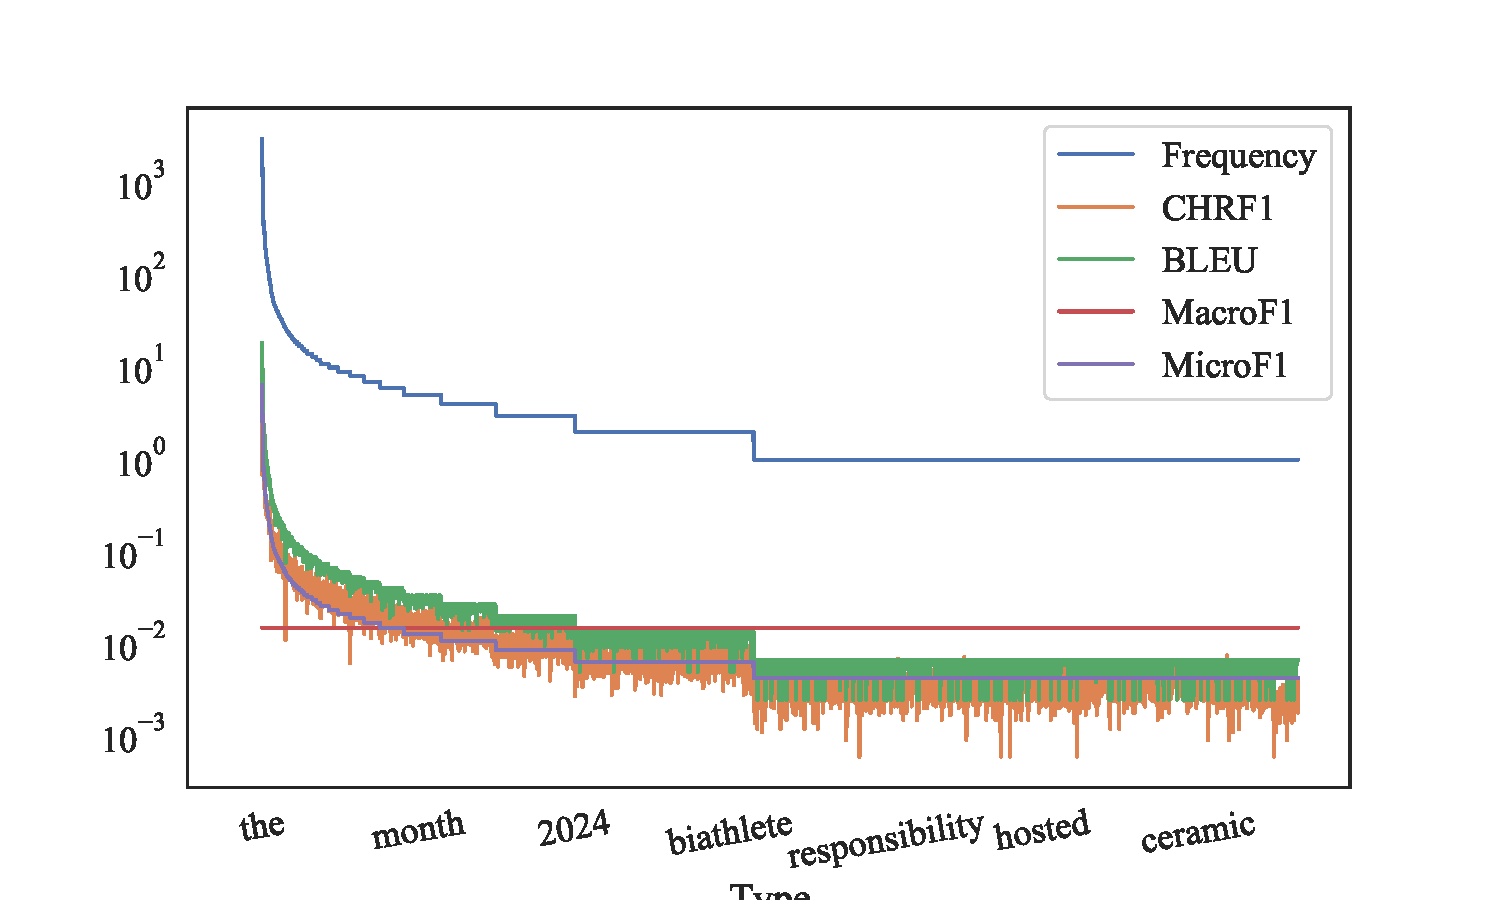
\includegraphics[width=\linewidth,trim={15mm 5mm 25mm 15mm},clip]{img/bleu-chrf-macro-micro-norecall.pdf}
%     \caption{\small Individual word type contribution to the corpus-level MT autoeval methods. % as measured on WMT NewsTest2019 German-English reference corpus.
%     The horizontal axis contains word types ranked by frequencies.
%     The vertical axis, which is in logarithmic scale, represents type frequencies (raw count) and percentile of contribution to the total corpus-level score. 
%     The contribution of a type is defined as the difference in corpus-level score between when the type is perfectly learned versus when it is fully ignored~(i.e zero-recall). 
%     %Perfect translations are simply when reference is treated as hypothesis where are as the full-ignorance or zero-recall is simulated for each type by replacing an out-of-vocabulary token of similar character count in the perfectly translated hypothesis~(therefore, no effect on length penalty).
%     %The roughness in lines of \bleu\ is and \chrf1 is due to the variation in n-grams affected by a type.
%     \mif1 uses only unigrams and scales the contribution by its frequency, whereas
%     \maf1, which is the focus of this work, is unweighted and assigns equal importance to all the types regardless of their frequencies. 
%     It is evident that the type contribution in \bleu\ and \chrf1 is scaled according to their frequency in the similar manner as \mif1.
%     For instance, `the' type appears 3019 times in the chosen test set, and zero-recall of `the' can result in loss up to 18.83\%, 9.38\%, 6.45\%, and 0.03\% of overall score in \bleu, \chrf1, \mif1, \maf1, respectively on the corpus used.
%     %Take away: \maf1 underscores the types on Long Tail where as others assign greater importance to the frequent words.
%     %Both \maf1 and \mif1 are described in detail in Section~\ref{sec:mt-cls-eval}.
%     }
% \label{fig:bleu-damage}
% \end{figure}



Our contributions are as follows:
We consider MT as a classification task, and thus admit \maf1 as a legitimate approach to evaluation~(Section ~\ref{sec:mt-as-cls}). 
We show that \maf1 is competitive with other popular methods at tracking human judgments in translation (Section~\ref{sec:wmt-metrics}). 
We offer an additional justification of \maf1 as a performance indicator on adequacy-focused downstream tasks such as cross-lingual information retrieval (Section \ref{sec:clir}). 
Finally, we demonstrate that \maf1 is just as good as the expensive BLEURT at discriminating between structurally different MT approaches in a way \bleu\ cannot, especially regarding the adequacy of generated text, and provide a novel approach to qualitative analysis of the effect of metrics choice on quantitative evaluation (Section \ref{sec:unmt}).

